\chapter{Sentimentanalyse}
\markright{\thechapter \,\,\currentname \, - Philipp Kappus}
\label{chap:sentiment}
Die Sentimentanalyse ist ein Teilgebiet des \gls{Text Mining} und beinhaltet die Klassifizierung von Aussagen und Meinungen in Texten in Kategorien wie z.B. "`positiv"'' und "`negativ"'\footfullcite[][S. 113]{python-sm-analysis}. Wie in Abschnitt \ref{sec:hypothesen} beschrieben, soll der Versuch unternommen werden, die gesammelten Tweets auf ihre Meinung mittels Sentimentanalyse zu untersuchen und daraufhin in Gruppen mit gleichen Werten zu klassifizieren. 
\section{Technologieauswahl}
\label{sec:Technologieauswahl}
Sentimentanalyse ist ein komplexer Vorgang, der Technologien aus dem Gebiet des \ac{NLP}, der Computerlinguistik und der Biometrik beinhaltet, weshalb hier auf schon existente Systeme zurückgegriffen wurde.
Bestehende Tool unterscheiden sich in Qualität der Analyse, Differenzierung der Einteilung (können einzelne Emotion extrahiert werden?) und Preis. 
Mit einer Datenbasis von ca. 10.000.000 Texten fallen alle kostenpflichtigen System aufgrund des begrenzten Budget aus, weshalb  die \gls{OpenSource} Systeme "`TextBlob"' und "`NLTK - Vader"' verwendet wurden. Damit kann jedem Tweet folgende drei Werte zugeordnet werden.
\begin{enumerate}
	\item $NLTK - Polarität \in [-1;1]$\\ Ein Maß für die Stimmung des analysierten Textes\\ wobei $-1\,\hat{=}\,max.\,negativ,\,1\,\hat{=} \,max.\,positiv$ 
	\item $TextBlob - Polarität \in [-1;1]$
	\item $TextBlob - Subjekivität \in [0;1]$\\ Ein Maß für die Objektivität des analysierten Textes\\ wobei $0\,\hat{=}\,max.\,objektiv,\,1\,\hat{=} \,max.\,subjektiv$ 
\end{enumerate}

Beide Systeme sind optimiert für englische Texte; bedeutet, alle gesammelten Tweets müssen vor der Analyse übersetzt werden. Im Bereich der maschinellen Übersetzung steigern sich die Kosten der Prozessierung der Datenbasis über das Budget weshalb eine Übersetzung aller Tweets nicht möglich war.
Allerdings konnten Tweets von 4 Tagen (01 - 04 März 2021)  übersetzt werden um anschließend eine Sentimentanalyse durchzuführen.

\section{Analyse}
\label{sentiment-daten-analyse}
Die Datenauswahl wurde mit den in Abschnitt \ref{sec:Technologieauswahl} genannten Tools analysiert. Dabei zeigten sich die Probleme der Sentimentanalyse:

Probleme der Erkennung von doppelten Verneinung oder Ironie treten auf oder von Menschen intuitiv als negativ betrachtetete Tweets werden falsch eingruppiert.
So z.B. an diesem Beispiel:\\
\textit{"`Wir brauchen keine "`Maßnahmen"' wegen einem Virus von vielen! Wir haben ein Immunsystem! Wir wollen raus aus dieser Matrix des Corona-Hoax! STOP THE GREAT RESET, er dient nicht unserer Gesundheit! Ganz bestimmt nicht!"'}\footfullcite{negativ-tweet} \\beinhaltet eine von Menschen eher als negativ aufgefasste Aussage. Trotzdem bewertet TextBlob die übersetzte Version mit einer Polarität von 0.659 und NLTK sogar mit 0.8. \\
Des Weiteren belastet die Covid-19 Pandemie  die meisten Nutzer*innen, sodass ein allgemein eher negativer Tonus in den Texten herrscht; das macht eine Unterscheidung schwierig.\\ 
Eine Einteilung in positiv und negativ ist oft nicht ausreichend, eine Unterscheidung z.B. zwischen politischen Gruppierungen ist nicht möglich.
Dafür bedarf es höher entwickelte Systeme die Aussagen bezüglich ihres Inhalts differenziert kategorisieren können.\\
Nichtsdestotrotz, wurde nach Gruppen von Nutzer*innen gesucht, die sich in ihren Sentimentwerten ähneln. 
Dafür wurde für jede*n Nutzer*in der Durschnittswert seiner/ihrer Sentimentwerte berechtet und diese Nutzer*innen anschließend als Punkte in einem dreidimensionalen Graph dargestellt.
\begin{figure}[h!]
	\centering
	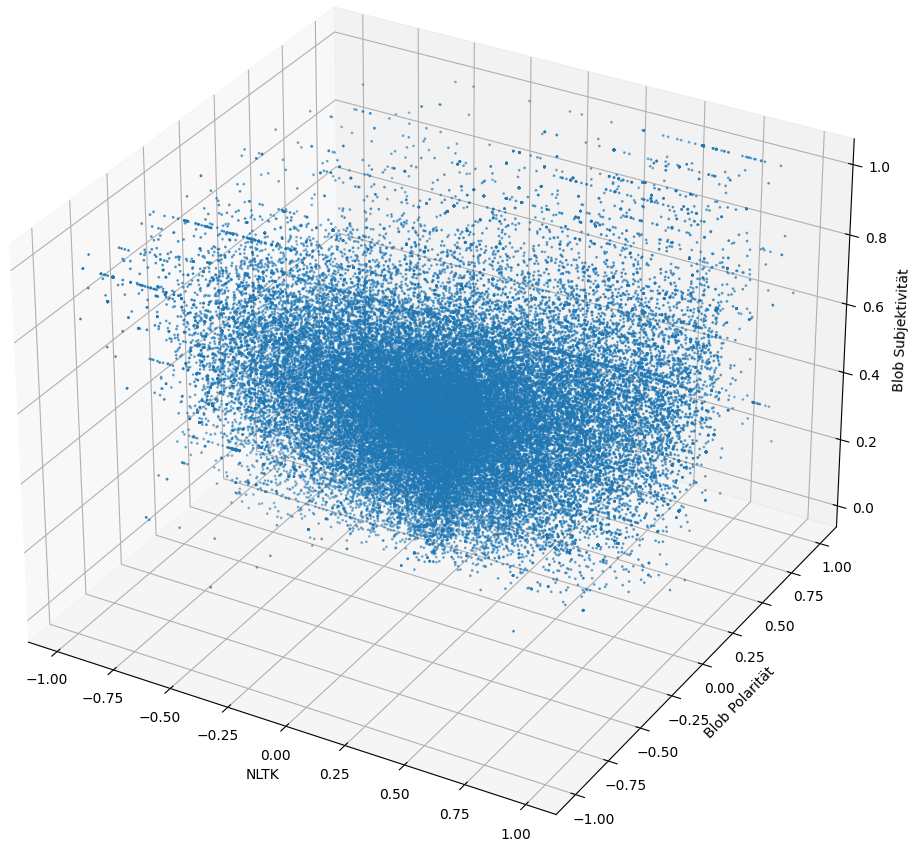
\includegraphics[width=0.5\linewidth]{images/SentimentPlot}
	\caption[]{Verteilung der Nutzer*innen anhand der durchschnittlichen Sentimentwerte ihrer Tweets}
	\label{fig:sentimentplot}
\end{figure}

In Abbildung \ref{fig:sentimentplot}  liegt eine unstrukturierte Verteilung vor, es sind keine offensichtlichen Gruppierung erkennbar.
Aufgrunddessen und weil der Datensatz aufgrund der Übersetzungs-Schranke nur schwer erweiterbar ist, sowie vor dem Hintergrund der oben genannten Ungenauigkeiten wurde der Versuch der Eingruppierung anhand von Sentimentdaten beendet.
